\chapter{Methodology and Data Analysis}

 Our primary intention was to conduct an in-depth qualitative analysis, focusing on gathering detailed, narrative data. However, as we delved into relevant literature and reviewed established methodologies, it became evident that a mixed-methods approach would be more effective in addressing the complexity of the research questions. Consequently, we developed a survey that included both qualitative and quantitative elements, providing a broader range of data to inform our analysis. To complement the survey findings, a personal interview with a key participant in the supply chain sector was conducted, enriching the qualitative aspect of our study.

To further refine and explore our research questions (RQs), we considered various methodological approaches, guided by the insights of \textcite{Ghauri2020ResearchStudies}. Ultimately, we designed a comprehensive questionnaire incorporating a mix of Likert-scale questions \parencite{Joshi2015LikertExplained,Batterton2017MilitaryIt,Mirahmadizadeh2018DesigningData} and yes/no questions to test our hypotheses. Additionally, we included a free-text section in the survey, encouraging respondents to provide detailed recommendations and observations beyond the structured questions. This open-ended question proved invaluable for the qualitative analysis, offering nuanced insights that supported our overall findings. Eventually we conducted a one-to-one interview with an experienced person from the industry to gether further personal insights. The combination of these approaches allowed for an investigation into supply chain resilience, blending quantitative aspect with qualitative depth. Here we will discuss in detail our entire research process and subsequently the methodology.

\section{Research Process}

Given that the pandemic had ended approximately three years prior to the initiation of this study, we recognized an opportunity to gather insightful data on supply chain adaptations and learnings from this global disruption. Our research approach combined both qualitative and quantitative methods to offer a comprehensive analysis of the pandemic's impact and the subsequent strategic responses of companies. This section outlines the research process in detail, describing each step taken from the initial conceptualization to the final analysis and presentation of findings.

\subsection{Initial Conceptualization and Literature Review}

The research process began with an initial idea to explore the intersection of the COVID-19 pandemic and supply chain management, driven by the awareness that three years after the pandemic, sufficient data might be available to gain valuable insights. The focus was on understanding the specific impact on perishable goods, which are characterized by their limited shelf life and essential nature. Given the changes in consumption patterns—where consumers were reluctant to shop in person but still needed essential items like groceries—we saw an opportunity to investigate how the supply chain for perishable goods was managed during such a crisis.

To frame the study, we conducted an extensive literature review, beginning with an overview of the pandemic's effects on supply chains and moving towards a more focused examination of resilience in supply chain management. This review helped us identify gaps in the existing literature and sharpen our focus on the perishable goods sector. From this, we formulated our research questions and hypotheses, aiming to understand both the immediate impacts of COVID-19 on supply chains and the strategies employed to enhance resilience and preparedness for future disruptions.

\subsection{Development of Research Questions and Hypotheses}

Based on the insights gathered from the literature review, we identified a research gap related to the strategic responses of suppliers of perishable goods during the COVID-19 pandemic. This led to the formulation of our research questions and hypotheses, which centered around whether suppliers faced significant disruptions, the nature of these disruptions, and the extent to which new strategies were implemented to enhance resilience. The hypotheses aimed to examine both the impact of the pandemic on supply chains and the strategic measures taken by suppliers to mitigate these impacts.

%=====================
\subsection{Deciding the approach}

The research aimed to adopt a quantitative approach to examine the impact of COVID-19 on the supply chain of perishable goods. We anticipated that sufficient data would be available to facilitate a robust quantitative analysis. Our objective was to obtain datasets that would allow us to compare variables such as sales, distribution, and buying patterns for perishable goods during the pandemic with the same variables before the pandemic. This approach was expected to provide a comprehensive understanding of the changes and disruptions experienced by supply chains in response to the pandemic. We began by searching for publicly available datasets that included sales and distribution data for perishable goods. For example, we sought data from grocery stores or companies, such as daily sales figures before, during, and after the pandemic, to analyze shifts in consumer buying behavior. 

Similarly, we aimed to collect data on the distribution of perishable goods to identify changes in logistics and supply chain practices during the pandemic period. However, our efforts to find complete datasets proved challenging. While we found various publicly available datasets, they often lacked critical components required for a meaningful comparative analysis. For instance, some datasets only covered periods before the pandemic, while others provided data exclusively for the post-pandemic period. Moreover, even when datasets included information for both before and after the pandemic, they frequently lacked data for the crucial period during the pandemic itself. Additionally, certain data we encountered, such as the Tesco grocery sales data, did not align with the specific time frames we needed for analysis. These gaps and inconsistencies in the available datasets hindered our ability to construct a valid and comprehensive quantitative analysis.

After numerous attempts and extensive searches, it became evident that we could not obtain the complete datasets required to perform a reliable quantitative comparison. Recognizing the limitations of continuing with this approach, we decided to pivot towards a qualitative methodology, in conjunction with quantitative approach when analysing the survey. This shift allowed us to explore the research questions from a different angle, focusing on gaining deeper insights into the experiences and perspectives of supply chain professionals during the pandemic. At this stage, we then began the preparation of the questions for survey based on the literature review and knowledge gathered so far.

%=====================

\subsection{Data Collection and Preliminary Analysis}

The next step involved collecting data to analyze the formulated hypotheses. The data collection began with the creation of survey questions informed by our literature review. These questions included both objective (yes/no or Likert scale responses) and subjective open-ended questions to capture a range of insights from industry professionals. We distributed the interview questions to potential participants via social media, professional networks, and direct email invitations. The responses collected provided a preliminary data set for analysis. We conducted a Partial Least Squares Structural Equation Modeling (PLS-SEM) analysis to evaluate the responses to the objective questions, enabling us to identify initial patterns and relationships. Simultaneously, we conducted a keyword analysis on the subjective responses to identify frequently mentioned themes and concepts. This analysis aimed to uncover underlying insights and patterns that might not have been immediately apparent from the quantitative data alone.

\subsection{Iterative Process and Refinement of Research Approach}

Despite obtaining some initial insights, the results from the PLS-SEM analysis were not conclusive enough to confidently establish or reject our hypotheses. Recognizing the need for deeper investigation, we decided to refine our approach. We conducted a more detailed analysis of the keyword data to understand what additional information was required to address our research questions more effectively. Based on this refined understanding, we developed a new set of more detailed, subjective questions for a long-form, one-to-one interview format. This approach was intended to elicit richer, more nuanced responses and to address specific areas of ambiguity or uncertainty identified in the preliminary analysis.

\subsection{In-Depth Interview and Analysis}

The next phase involved identifying and securing a participant with substantial experience in supply chain management for perishable goods to conduct a comprehensive in-depth interview. After several attempts to reach out through professional networks, we successfully arranged an interview with a suitable candidate. The interview was conducted in a one-on-one format, allowing for a thorough exploration of the interviewee’s experiences and insights related to supply chain resilience during the pandemic. Following the completion of the in-depth interview, we conducted a qualitative analysis of the responses. This analysis was carried out using thematic coding and contextual examination, allowing us to correlate the findings with the initial quantitative data and to further explore the emergent themes. By integrating the qualitative insights with the findings from the PLS-SEM analysis and the keyword analysis, we developed a more comprehensive understanding of the strategies implemented by suppliers during the pandemic.

\subsection{Presentation of Research Findings}

Finally, the research findings were compiled and presented in the subsequent sections of this thesis. Each stage of the research process contributed to a deeper understanding of the impacts of COVID-19 on supply chain resilience for perishable goods and the strategic responses implemented by suppliers. Further details of each step, including the methods, analyses, and findings, are elaborated in the following sections.

\noindent The entire process is also demonstrated in the Figure \ref{fig:research_process}.

\begin{figure}[H]
  \centering
  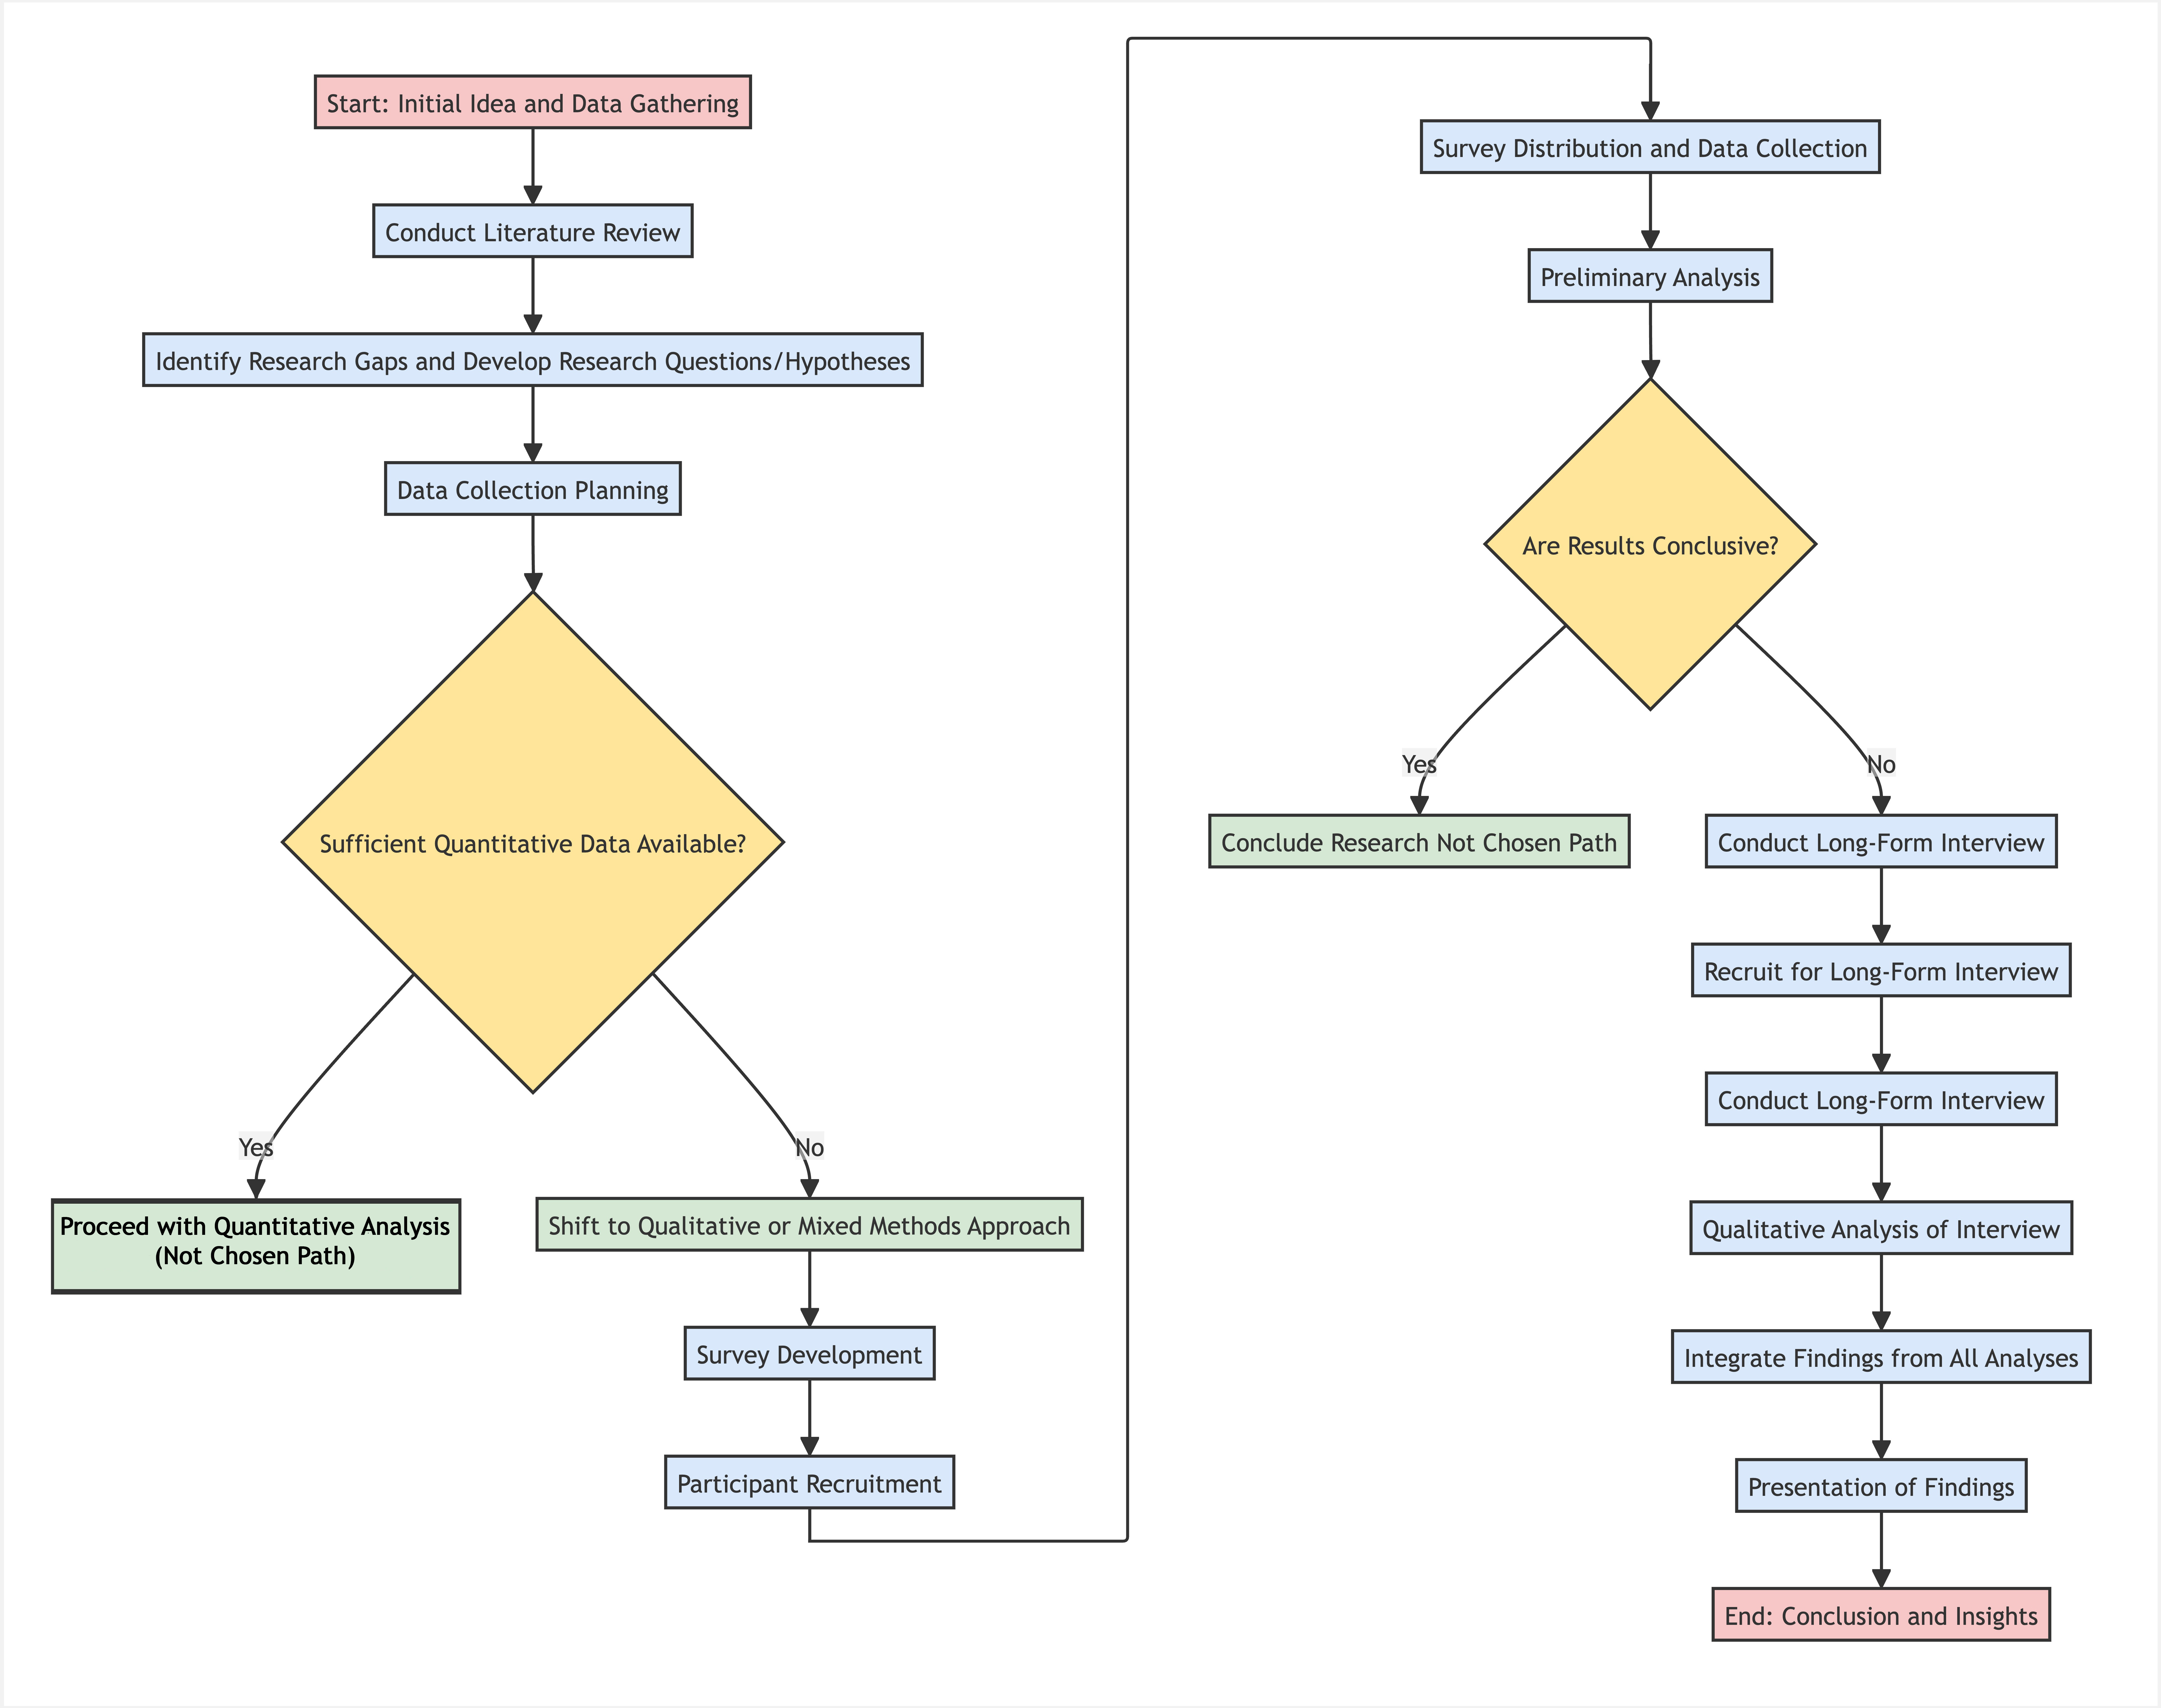
\includegraphics[width=1\textwidth]{figure/research_process.jpg}
  \caption{The research process.}
  \label{fig:research_process}
\end{figure}

\section{The Survey}

\subsection{Format of the survey}
In designing our survey for this study, we utilized a combination of Likert scale questions, yes/no questions, and a single subjective question, as previously mentioned. The Likert scale, a fundamental tool in social science research, was particularly useful for quantifying attitudes, beliefs, and behaviors related to supply chain resilience during the COVID-19 pandemic. By converting qualitative perceptions into quantitative data, it allowed us to perform a robust statistical analysis of these subjective constructs. While Likert scales can vary in length, we chose a 5-point scale (ranging from Strongly Agree to Strongly Disagree) to simplify the process for our respondents, thereby reducing their burden and encouraging higher completion rates. 

Our approach involved careful consideration of the number and type of questions included in the survey. Although it is common to use extensive Likert-scale questionnaires for detailed statistical analysis, we opted to limit the number of these questions to three, recognizing the low response rate and the need to maintain participant engagement. This decision was influenced by the initial literature review, which indicated that reducing the complexity of the survey could lead to more reliable data collection. The yes/no questions were strategically included to provide clear, straightforward insights into whether companies had implemented measures to address specific supply chain challenges, without delving into the success or failure of those measures. To develop the Likert scale questions, we conducted a thorough review of current topics in supply chain management, with a focus on resilience and challenges during the pandemic, as highlighted in several key publications. These questions were designed to be clear, concise, and free from bias, each aiming to capture the respondents' level of agreement or disagreement with statements reflecting critical aspects of their internal processes. 

The layout of our survey was meticulously crafted to minimize confusion and bias. We ensured that instructions were clear and emphasized that there were no right or wrong answers, which was crucial for maintaining the anonymity and confidentiality of respondents. This approach was intended to foster honest and thoughtful responses. The inclusion of a single open-ended question at the end of the survey allowed participants to provide additional insights or recommendations, adding a qualitative dimension to our analysis. In terms of administration, the survey was conducted online to maximize reach and convenience, given the constraints of the pandemic. This method was chosen to increase the response rate and ensure that we collected a representative sample. The combination of Likert scale questions with yes/no questions provided a comprehensive view of supply chain resilience, allowing us to understand not only the existence of specific measures but also the attitudes and thought processes behind them. This mixed-method approach ultimately provided a nuanced understanding of the challenges faced by supply chains during the pandemic.

\subsection{Survey Design and Rationale}

The survey developed for this study was meticulously designed to capture a comprehensive understanding of the impact of the COVID-19 pandemic on supply chain resilience, particularly within the context of perishable goods. Each question was carefully crafted to elicit specific insights while allowing for future in-depth analysis based on the data collected. The rationale behind the selection and formulation of each question reflects our intent to gather both quantitative and qualitative data that can inform broader discussions on supply chain strategies and their efficacy during unprecedented disruptions.

\subsubsection*{Identification of Perishable Goods}
The initial question aimed to categorize the type of perishable goods managed by the respondents' companies. Recognizing the diversity in perishable goods—ranging from vegetables and dairy products to meat, poultry, and seafood—this question was essential for contextualizing the subsequent responses. By allowing participants to select multiple categories, the survey accounted for companies dealing in various types of perishable goods. This categorization facilitated the understanding of industry-specific challenges and also enabled potential comparative analysis across different types of perishable goods. Defining "perishable goods" within the survey ensured that all participants had a consistent understanding, thereby reducing any ambiguity in their responses.

\subsubsection*{Company Turnover and Size}
The subsequent questions concerning the company’s turnover and size were designed to explore the potential correlation between a company’s scale and its response to supply chain disruptions. The turnover question was included to differentiate between small, medium, and large enterprises, allowing us to assess whether financial resources influenced the effectiveness of supply chain strategies during the pandemic. Larger companies, with their broader reach and potentially more complex supply chains, might have different strategies compared to smaller firms with more localized operations. This question set the stage for analyzing whether the scale of operations impacted a company’s ability to adapt to the pandemic-induced challenges. Similarly, the question regarding company size, classified into small (up to 50 employees), medium (51-250 employees), and large enterprises (over 250 employees), was intended to further refine our understanding of how organizational structure and capacity might influence supply chain resilience. By capturing this data, we anticipated the ability to segment responses and explore trends that might differ based on the size of the organization. For instance, larger enterprises might have more formalized strategies and resources, while smaller companies might rely on more agile and ad-hoc approaches.

\subsubsection*{Supply Chain Disruptions and Strategic Responses}
A critical component of the survey involved assessing the extent to which the COVID-19 pandemic disrupted supply chains, specifically for perishable goods. This question utilized a Likert scale, ranging from 1 (not at all) to 5 (very significantly), to capture the severity of the disruption as perceived by the respondents. The use of a Likert scale in this context allowed for a nuanced understanding of the impact, enabling respondents to express varying degrees of disruption. This data is crucial for understanding the scale of the challenge faced by different companies and sets the foundation for analyzing how these disruptions influenced subsequent strategic decisions. Following this, the survey inquired whether the company had implemented any changes to its supply chain strategies during the pandemic. This yes/no question aimed to capture a binary response, providing a clear indicator of whether companies actively adapted their supply chain practices in response to the crisis. This question was followed by another yes/no question regarding whether companies had diversified their supplier base—a common strategy to mitigate risks associated with supply chain disruptions. The sequential nature of these questions was intentional, designed to lead respondents from the recognition of disruption to specific strategic responses, thus creating a logical flow in the survey.

\subsubsection*{Evaluating the Effectiveness of Resilience Strategies}
The survey then probed the effectiveness of the resilience strategies that were in place before the pandemic. Using a Likert scale from 1 (not effective) to 5 (extremely effective), this question sought to gauge how well-prepared companies were to handle the unprecedented challenges posed by the pandemic. By asking participants to evaluate the success of their existing strategies, the survey aimed to identify potential gaps in preparedness and areas where companies may have over or underestimated their resilience. Further, the survey explored whether companies had developed any backup plans for future disruptions. This question, also structured as a yes/no option, was critical in understanding the lessons learned by companies during the pandemic and whether they had proactively taken steps to bolster their supply chain resilience against future crises. The inclusion of this question allowed us to assess the forward-thinking approaches of companies and their commitment to improving resilience post-pandemic.

\subsubsection*{Adjustments in Demand Forecasting and Pandemic Preparedness}
The survey also addressed whether companies had adjusted their demand forecasting methods in response to the pandemic. Accurate demand forecasting is pivotal in supply chain management, especially in times of uncertainty. The question sought to determine if companies had recognized the need for more adaptive forecasting techniques as market conditions rapidly changed during the pandemic. The final structured question asked whether the company had established a formal pandemic preparedness plan for future events. This yes/no question aimed to determine whether the experiences of the COVID-19 pandemic had led to the institutionalization of specific preparedness measures. The presence of such a plan would indicate a company’s strategic shift towards long-term resilience and readiness for potential future disruptions.

\subsubsection*{Subjective Insights from Participants}
To complement the structured questions, the survey included a subjective, open-ended question inviting respondents to share additional insights based on their personal experience of handling supply chain issues during the pandemic. This question was strategically placed at the end of the survey to provide participants with the opportunity to elaborate on any points not covered by the structured questions. It allowed for the collection of qualitative data that could offer deeper insights into the challenges and strategies employed by different companies. This open-ended format included to capture the unique perspectives and innovative solutions that may not have been addressed through the more structured questions.

\subsection{Survey Distribution and Targeting}

The survey for this study was created using Google Sheets, allowing us to generate a shareable link that could be easily distributed to potential participants. The complete set of survey questions can be found in Appendix \ref{appendix:survey}. The focus of our work was narrowed to contain only European countries as we, the authors, are located in European Union member countries and found that this demographic affects us the most. Our focus was exclusively on participants from Europe, reflecting our research's geographic concentration. To identify suitable participants, we conducted extensive research on LinkedIn. We filtered potential contacts by country and then searched for individuals holding prominent positions relevant to supply chain management, such as Purchasing Assistant, Store Manager, Location Manager, and Director of Procurement, among others. 

This approach enabled us to target professionals directly involved in supply chain operations across various European countries. The companies selected were among the top 5 chain supermarkets in countries with the highest GDP in the Union. Some of the countries selected are such but not limited to Sweden, Norway, Czech Republic, the Netherlands, England, Spain, Germany, and etc. This ensured that we take samples of countries with different Geo-locations. As can be seen, some countries are Nordic, which are larger landmass countries with scarcely populated cities, where other countries such as the Netherlands, Spain, and France are evenly populated or almost densely populated areas. 

After identifying potential participants on LinkedIn, we initiated contact primarily through LinkedIn messaging. In cases where contact details were not readily available, we supplemented our efforts by sending emails. For those whose emails were not publicly available, we employed a common email format (first name dot last name at the company's domain) to reach out to them. We ensured that participants were informed that their responses would remain anonymous, with no personal details being recorded. This information was clearly communicated in both the LinkedIn messages and emails sent to potential respondents. 

Additionally, we emphasized that participation in the survey was entirely voluntary, with no mandatory questions. This approach was designed to make it easier for participants to complete the survey, even if they chose not to answer every question. Understanding that respondents might be reluctant to spend significant time on surveys, we streamlined the process by designing the entire survey to fit on a single page, eliminating the need for a "next" button. Despite the absence of incentives such as prize money or other benefits, we encouraged participation by emphasizing the importance of their input in our research. In total, we targeted participants from 16 European countries and successfully contacted approximately 275 individuals across a range of supermarkets, including Netto, Coop, Lidl, Kiwi, Aldi, Carrefour, and more. For a detailed breakdown of the number of people contacted, the countries involved, the supermarkets represented, and the typical positions targeted, please refer to Table \ref{tab:survey-participants}.



\begin{table}[H]
\scriptsize
\centering
\begin{tabular}{@{}|l|l|l|l|@{}}
\toprule
\textbf{Country} & \textbf{\begin{tabular}[c]{@{}l@{}}Number of \\ People \\ Contacted\end{tabular}} & \textbf{Supermarkets}                                                                                          & \textbf{Positions}                                                                                                                                                                                             \\ \midrule
Sweden           & 43                                                                                & \begin{tabular}[c]{@{}l@{}}Citigross, Martin \& Cervera, \\ Coop, Hemshop, ICA, Willys, \\ Mathem\end{tabular} & \begin{tabular}[c]{@{}l@{}}Store Manager, Purchasing Assistant, \\ Location Manager, Purchasing \\ Manager, Perishable Purchaser\end{tabular}                                                                  \\ \midrule
Norway           & 9                                                                                 & Kiwi, Coop                                                                                                     & \begin{tabular}[c]{@{}l@{}}Store Manager, Purchaser, Head of \\ Indirect Procurement, Senior \\ Strategic Buyer\end{tabular}                                                                                   \\ \midrule
Denmark          & 19                                                                                & Netto, Coop, Lidl                                                                                              & \begin{tabular}[c]{@{}l@{}}Senior Buyer, Category Manager, \\ Purchasing Assistant, \\ Category Director\end{tabular}                                                                                          \\ \midrule
Finland          & 4                                                                                 & S-Market, K-Supermarket, Lidl                                                                                  & \begin{tabular}[c]{@{}l@{}}Junior Purchasing Manager, \\ Purchasing and Sales Director\end{tabular}                                                                                                            \\ \midrule
Belgium          & 19                                                                                & Aldi, Carrefour, Lidl, Colruyt                                                                                 & \begin{tabular}[c]{@{}l@{}}Senior Buyer, Head of Sales \\ and Purchasing, Technical \\ Purchasing Manager, Reverse \\ Logistics Manager\end{tabular}                                                           \\ \midrule
Netherlands      & 15                                                                                & Albert Heijen, Aldi, Lidl                                                                                      & \begin{tabular}[c]{@{}l@{}}Manager Procurement, \\ Purchasing Manager, \\ Senior Director Procurement\end{tabular}                                                                                             \\ \midrule
Spain            & 34                                                                                & \begin{tabular}[c]{@{}l@{}}Marchedona, Carrefour, Lidl, \\ Aldi, Supercore\end{tabular}                        & \begin{tabular}[c]{@{}l@{}}CSR Manager, IT Procurement \\ Manager, Senior Buyer, Indirect \\ Purchasing VP, \\ Supply Chain Manager\end{tabular}                                                               \\ \midrule
Portugal         & 18                                                                                & \begin{tabular}[c]{@{}l@{}}Pingo Doce, Continente, \\ Intermarche\end{tabular}                                 & \begin{tabular}[c]{@{}l@{}}Category Manager, National Retail \\ Operations Director, Store Manager, \\ Digital Channels Director\end{tabular}                                                                  \\ \midrule
France           & 18                                                                                & \begin{tabular}[c]{@{}l@{}}Carrefour, Intermarche, \\ Monoprix\end{tabular}                                    & \begin{tabular}[c]{@{}l@{}}Global Category Management, \\ International Head of Buying, \\ Import Director, Director of \\ Supply Chain, Trader\end{tabular}                                                   \\ \midrule
Greece           & 9                                                                                 & \begin{tabular}[c]{@{}l@{}}Sclavenitis, Alpha Beta \\ Vassilopoulos\end{tabular}                               & \begin{tabular}[c]{@{}l@{}}Category Manager, Buyer, Logistic \\ Project Manager, Warehouse Manager\end{tabular}                                                                                                \\ \midrule
Switzerland      & 27                                                                                & Denner, Migros, Aldi                                                                                           & \begin{tabular}[c]{@{}l@{}}Logistic B. Denner, Product \\ Manager, Senior Group Category \\ Director, Buying Director, Country \\ Managing Director, Manager, \\ National Supply Chain Management\end{tabular} \\ \midrule
Italy            & 20                                                                                & \begin{tabular}[c]{@{}l@{}}Conad, Gruppo Selex, \\ Eurospin\end{tabular}                                       & \begin{tabular}[c]{@{}l@{}}Category Manager, Director Supply \\ Chain, National Category Manager, \\ Logistics Manager, Buyer, \\ Logistics Specialist\end{tabular}                                            \\ \midrule
Austria          & 14                                                                                & Rewe, Hofer                                                                                                    & \begin{tabular}[c]{@{}l@{}}Senior Category Manager, Head of \\ Shift Logistic, Procurement Manager, \\ Buying Manager, Buying Specialist, \\ Group Director at Supply \\ Chain Management\end{tabular}         \\ \midrule
Czech Republic   & 10                                                                                & Albert, Tesco                                                                                                  & \begin{tabular}[c]{@{}l@{}}Head of Supply Chain, Supply Chain \\ Manager, Director of Strategic Sourcing, \\ Buying and Merchandising Director\end{tabular}                                                    \\ \midrule
Poland           & 13                                                                                & Eurocash, Zabka                                                                                                & \begin{tabular}[c]{@{}l@{}}Supply Chain Planning Manager, \\ Senior Supply Chain Manager, \\ Logistics Controlling Manager, \\ Logistics Operation Manager\end{tabular}                                        \\ \midrule
Slovakia         & 3                                                                                 & Tesco                                                                                                          & \begin{tabular}[c]{@{}l@{}}Stock Controller Coordinator, \\ Big Data Analyst for Supply \\ Chain, Supply Chain Promotion Manager\end{tabular}                                                                  \\ \bottomrule
\end{tabular}
\caption{Number of people contacted for the survey. Total number of contacts - 273. Total responses - \participantCount}
\label{tab:survey-participants}
\end{table}

When we encountered challenges in gathering sufficient responses for our study on supply chain resilience, especially from experts in specialized fields, we found that a multi-faceted approach was necessary. We expanded our reach by leveraging our extended professional networks through platforms like LinkedIn. We urged our first or second circle contacts to reach out to their contacts and help us with the surveys and finally, we picked up the phone and tried to reach those individuals through company reception numbers and cold-calling professionals at their office numbers within our local country and beyond. Additionally, we utilized  social media forums and professional networks to connect directly with potential participants.  These strategies significantly enhanced our ability to collect the necessary data efficiently  enabling the accumulation of sufficient data to conduct a substantive analysis, ensuring that the qualitative research met statistical validity and reliability criteria.

% \label{sec:pls-sem}

\subsection{Methodology for Survey Analysis}

Data analysis is a critical component of research across various domains, providing essential insights and driving informed decision-making. As data complexity and volume continue to grow, so does the need for sophisticated techniques to analyze and interpret this data effectively. This section explores several prominent data analysis techniques used in contemporary research, followed by an in-depth discussion of Partial Least Squares Structural Equation Modeling (PLS-SEM). We will conclude with a rationale for choosing PLS-SEM as the most suitable method for our thesis. 

\subsubsection{Data Analysis Techniques}

The field of data analysis encompasses a wide range of techniques and methods designed to extract meaningful insights from complex datasets. These techniques serve various analytical purposes, from understanding fundamental patterns in data to developing sophisticated predictive models. Given the diversity of data types, research objectives, and contexts in which data is analyzed, selecting the appropriate method is crucial for achieving reliable and valid results. This section provides a concise overview of several key data analysis techniques commonly employed in academic and professional research. Each method offers unique advantages and is suited to specific types of data and research questions, contributing to the robust analysis and interpretation of data in various domains.

\begin{description}[font=\normalfont\itshape]
    \item[\textit{\textbf{Descriptive Statistics}}] Descriptive statistics provide a foundational understanding of data by summarizing its main characteristics through measures such as mean, median, mode, and standard deviation. These statistics are essential for preliminary data analysis, offering a snapshot of data distribution and variability \parencite{Mann2018IntroductoryStatistics}.

    \item[\textit{\textbf{Regression Analysis}}] Regression analysis is a powerful technique used to understand the relationship between dependent and independent variables. It includes various forms such as linear regression, logistic regression, and multiple regression, each serving specific analytical needs \parencite{Montgomery2021IntroductionAnalysis}.

    \item[\textit{\textbf{Factor Analysis}}] Factor analysis is used to identify underlying relationships between measured variables. It helps in data reduction by grouping variables into factors based on their correlations, making complex data more manageable and interpretable \parencite{Andy2018DiscoveringStatistics}.

    \item[\textit{\textbf{Cluster Analysis}}] Cluster analysis involves grouping a set of objects in such a way that objects in the same group (or cluster) are more similar to each other than to those in other groups. This technique is widely used in market research, pattern recognition, and bioinformatics \parencite{Hair2019WhenPLS-SEM}.

    \item[\textit{\textbf{Time Series Analysis}}] Time series analysis focuses on analyzing data points collected or recorded at specific time intervals. Techniques such as ARIMA and Exponential Smoothing are used to forecast future trends based on historical data \parencite{Box2015TimeControl}.

    \item[\textit{\textbf{Partial Least Squares Structural Equation Modeling (PLS-SEM)}}] \hfill \\
    PLS-SEM is a multivariate statistical analysis technique used to analyze complex relationships among variables. It is particularly useful for predictive modeling and theory building in situations where the data is not normally distributed or the sample size is small \parencite{Sarstedt2017PartialModeling}.
\end{description}

\subsubsection{PLS SEM for Research}

Partial Least Squares Structural Equation Modeling (PLS-SEM) is a powerful statistical technique and a second-generation multivariate method gaining traction in various research fields, particularly in social sciences, business research, marketing, and information systems. It allows researchers to construct and test complex models involving multiple latent and observed variables and is particularly useful for models with numerous variables, intricate relationships, and multiple indicators for each variable \parencite{Sarstedt2017PartialModeling, Henseler2015AModeling}. PLS-SEM helps researchers analyze the interplay between multiple variables, including those not directly measurable (latent variables), thereby providing a deeper understanding of cause-and-effect relationships in complex systems \parencite{Sarstedt2017PartialModeling}. Unlike Covariance-Based SEM (CB-SEM), PLS-SEM focuses on maximizing the explained variance of dependent constructs, making it an ideal choice for predictive modeling, theory development, and exploratory research \parencite{Chin1998TheModeling} \parencite{Sarstedt2017PartialModeling}. In contrast to techniques focused on confirming existing theories, PLS-SEM is particularly suited for developing new theories or extending existing ones, especially when the goal is to predict or identify key factors influencing a phenomenon \parencite{Chin1998TheModeling}. PLS-SEM thrives in contexts where data complexity is the norm, such as in studying intricate systems like family businesses or large-scale marketing campaigns \parencite{Henseler2015AModeling}. PLS-SEM's robustness and flexibility allow it to handle challenging data conditions that traditional methods may not manage effectively. It accommodates both reflective and formative measurement approaches, offering the flexibility to choose between indicators that either reflect or form the underlying concept, depending on the research question \parencite{Chin1998TheModeling}. 

This method is advantageous in dealing with real-world data that does not always follow a perfect normal distribution, making minimal assumptions about the underlying data distribution \parencite{Lohmoller1989LatentSquares}. It also supports the evaluation of theoretical models, even with smaller sample sizes, unlike other techniques that require larger samples for accuracy \parencite{Sarstedt2017PartialModeling}. The methodology has gained popularity in fields such as marketing, information systems, and social sciences due to its capacity to model intricate relationships and assess the reliability and validity of constructs, even with small samples and non-normal data distributions \parencite{Chin1998TheModeling}. 

It effectively tackles common challenges in social science research, making it particularly suitable for complex models where data may be limited or challenging to collect. Moreover, PLS-SEM has been highlighted as a robust solution in evaluating theoretical models in the social sciences, business research, and other fields where data complexity is prevalent \parencite{Sarstedt2017PartialModeling}.

PLS-SEM is well-suited for exploratory research and prediction-oriented studies due to its focus on maximizing the explained variance of the dependent variables \parencite{Henseler2015AModeling}. Unlike traditional covariance-based SEM methods, which often require larger sample sizes and confirmatory analysis, PLS-SEM provides a reliable alternative for research scenarios that demand flexibility and adaptability in dealing with diverse data structures and research objectives.

\paragraph{Key Features of PLS-SEM}

PLS-SEM prioritizes prediction, making it suitable for exploratory research where theory is less developed.It is capable of handling both reflective and formative measurement models \parencite{Chin1998TheModeling}. It is effective with small to medium sample sizes, which is often a limitation in other SEM approaches \parencite{Sarstedt2017PartialModeling}. It is robust against deviations from normality, allowing for broader applicability across different datasets \parencite{Henseler2015AModeling}. Additionally, PLS-SEM offers a valuable toolkit for researchers navigating complex relationships and data limitations. Its ability to handle intricate models, work with small samples, and provide flexibility in measurement makes it a compelling choice for various research endeavors \parencite{Tenenhaus2005PLSModeling}.

\paragraph{Steps in PLS-SEM}

\begin{itemize}
    \item \textbf{Model Specification}: Define the structural and measurement models. The structural model (inner model) specifies relationships between latent variables, while the measurement model (outer model) links latent variables to their indicators \parencite{Lohmoller1989LatentSquares}.

    \item \textbf{Model Identification}: Ensure the model is identified with sufficient data points to estimate parameters.

    \item \textbf{Data Collection}: Gather data for all observed variables.

    \item \textbf{Model Estimation}: Use the PLS algorithm to estimate path coefficients, weights, and loadings \parencite{Wold1985SystemsSquares}.

    \item \textbf{Model Evaluation}: Assess the model using criteria such as convergent validity, discriminant validity, composite reliability, and R² values \parencite{Tenenhaus2005PLSModeling}.

    \item \textbf{Model Interpretation}: Interpret the results to draw meaningful conclusions about the relationships between constructs.
\end{itemize}

\paragraph{Model Evaluation Criteria}

\begin{itemize}
    \item \textbf{Convergent Validity}: Assessed through Average Variance Extracted (AVE), which should exceed 0.50 \parencite{Henseler2015AModeling}.

    \item \textbf{Discriminant Validity}: Evaluated using the Fornell-Larcker criterion, where the AVE of each construct should be greater than the squared correlations with other constructs \parencite{Henseler2015AModeling}.

    \item \textbf{Composite Reliability}: Should be above 0.70 to ensure reliability of constructs \parencite{Sarstedt2017PartialModeling}.

    \item \textbf{R\textsuperscript{2} Values}: Indicate the amount of variance in the dependent variables explained by the model.
\end{itemize}

\paragraph{Motivation for Using PLS-SEM}

The choice of PLS-SEM for our research is motivated by several key factors that align with the nature of our dataset and research objectives. Our research model, while not overly complex, involves three key constructs that require a nuanced analysis of relationships and interactions. PLS-SEM is particularly suited for this type of model, as it allows us to efficiently explore the connections between these constructs without being restricted by the limitations of simpler modeling techniques. Moreover, our study seeks to understand the relationships between pandemic-induced disruptions, change management practices, and resilience strategies, necessitating a method that can simultaneously assess both the measurement model (which evaluates the reliability and validity of constructs) and the structural model (which examines the relationships between constructs). This dual focus is critical for addressing our research questions, particularly given our initial assumptions about the significance of resilience strategies prior to the survey.

Additionally, PLS-SEM offers flexibility in handling low variance data, which is particularly relevant given the minimal variance observed in our responses; traditional methods that depend on maximizing explained variance would not be suitable in this context. Instead, PLS-SEM enables us to model and interpret the structural relationships effectively, even when the variance explained by the model is low, emphasizing the estimation of path coefficients and identifying key drivers. The method's robustness to data and sample size constraints also makes it ideal for our study, as our dataset is moderately sized and may not meet the stringent requirements of other SEM techniques that rely on larger sample sizes and normal data distributions. Furthermore, PLS-SEM is particularly suited for exploratory research, allowing us to uncover new insights and develop theoretical models. Given that our primary aim was to explore potential relationships between constructs rather than confirm them definitively, PLS-SEM serves as an appropriate and reliable choice for our analysis.

\noindent In conclusion, PLS-SEM offers a valuable toolkit for researchers navigating complex relationships and data limitations. Its ability to handle intricate models, work with small samples, and provide flexibility in measurement makes it a compelling choice for various research endeavors \parencite{Tenenhaus2005PLSModeling}.

\subsection{Keyword Extraction for Open-Ended Question}

As discussed previously, we have introduced one open-ended question within our survey, namely: (Refer the entire questionnaire in Appendix \ref{appendix:survey}).

\begin{tcolorbox}[colback=blue!5!white, colframe=blue!15!black, boxrule=0.5mm, title=Subjective Question, fonttitle=\bfseries]
  We would really appreciate it if you can add some insights based on your personal experience of handling supply chain issues during the pandemic.
\end{tcolorbox}

Due to the nature of this question, a different approach was needed to analyse all the responses. While we have engaged in a thorough qualitative examination of the subjective responses—employing a traditional interpretative approach to manually read and derive inferences from the survey data—our analysis did not stop there. Recognizing the value of quantifiable insights in enhancing the reliability and generalizability of our findings, we subsequently applied statistical methods to analyze these responses. This dual approach enabled us to capture the nuanced perspectives offered by the respondents, and also to quantify patterns and trends that could be systematically validated. In this section we will discuss the quantitative methodology employed by us. 

There are various recognised methodologies that are used to analyse subject data. \textcite{Joshi2024AAnswers} have analysed various methodologies that are used to perform automated assessment for subjective responses as we have received in our questionnaire. Content Analysis \parencite{Harwood2003AnAnalysis}, which is a systematic technique for interpreting textual data by categorizing the content into various groups based on specific criteria. While it can be both qualitative and quantitative, often the frequency of words, phrases or topics are counted to identify patterns or trends. Another prominent methodology, Thematic Analysis \parencite{terry2017thematic} predominantly qualitative and focuses on identifying and analyzing patterns or themes within data. It involves closely reading the text to code data and sort these codes into themes that emerge organically. It's flexible and can uncover rich, detailed, and complex data interpretations. 

Discourse Analysis \parencite{gill2000discourse}, while defined differently in many literature, generally goes beyond the content of text to consider the context and means of communication. It examines how language is used in the text to convey messages, and how this relates to social and cultural contexts. In addition, another prominent method, Grounded theory \parencite{birks2015grounded_ch1} is used to generate or discover a theory through the data collected. It involves collecting data and analyzing it iteratively. As more data is collected, and analysis proceeds, the emerging theory or conceptual framework starts to take shape. This method is particularly useful for new areas of research where existing theories might not apply. Another prominent methodologies are Sentiment Analysis \parencite{Wankhade2022AChallenges}, Lexical Analysis \parencite{Bolden2000BridgingDivide}, Narrative Analysis \parencite{Burck2005ComparingAnalysis}, Machine Learning Techniques \parencite{Jain2021AReviews, Alantari2022AnReviews} and Keyword Extraction.

Keyword Extraction \parencite{Firoozeh2020KeywordMethods, Bharti2017AutomaticSurvey} is a broad umbrella that includes various automatic and manual methodologies that prominently focuses on extracting keywords from subjective texts. \textcite{Yuan2018TextStrategy} describe some prominent Keyword Extraction algorithms. TF-IDF (Term Frequency-Inverse Document Frequency) is about weighting the frequency of a word in a document against its frequency across all documents to identify its importance, while LDA (Latent Dirichlet Allocation) is a probabilistic model that identifies topics distributed across a corpus of texts and assigns keywords to these topics based on their distribution, furthermore, TextRank is a graph-based ranking model for text processing which forms a network from the text and uses the structure of this network to determine the importance of words or phrases. 

Building on the array of methodologies previously described for analysing textual responses, our approach used in this study diverges somewhat from conventional automated techniques. Insted of deploying established algorithms such as TF-IDF, LDA, or TextRank, we adopted a manual extraction method. This methodological choice was chosen on several key considerations. Firstly, the manageable scope of the dataset - comprising of \participantCount{} responses, each encapsulated within two to three sentences - rendered manual analysis both feasible and practical. This hands-on approach ensured we understand the overall theme of the response, and that we can perform nuanced comprehension and interpretation, which could easily be missed by employing any simple text parsing or word frequency analysis tools/algorithms. For instance, different respondents might articulate similar sentiments or ideas using disparate linguistic expressions, something that purely automated systems could potentially overlook. 

This manual method, could possibly be categorised, or partially categorised under various analytical paradigms. It shares affinities with \textit{content analysis} in its meticulous parsing of text to identify key terms; and with \textit{thematic analysis} in its sensitivity to underlying themes conveyed across all responses. This technique, however, does not align strictly with any single established methodology like \textit{sentiment analysis} or \textit{discourse analysis}, although it incorporates elements of these through its interpretative elements. The decision to abstain from fully automated methods was also taken due to the desire to preserve the integrity and depth of qualitative data, ensuring that the richness of the respondents' expressions was fully captured and reflected in the analysis. 

In our approach of keyword extraction, our methodology entailed a meticulous manual review of each response. We initiated this process by reading through the first entry comprehensively, extracting prominent keywords that capture the the essence of the respondents' perspectives. Some noteworthy keywords involve "\textit{diversified supplier base}", "\textit{demand forecasting}" and "\textit{strengthening supply ties}". This will be discussed in detail in further sections. It is important to note that the response need not contain the exact phrase of \textit{diversified supplier base}; however, if the respondent talks about diversifying their supplier base in any other way, we have used the a common and popular term that could explain their sentiments in our extraction. The same process is employed in extraction any other keywords from the answer. Subsequent to this extraction, we engage in an iterative review process, where we similarly analyse the next response. If this response discusses something that aligns with any of the existing keywords, we increase the frequency of those keywords by one, meanwhile also trying to extract any more prominent keywords from the response. We keep doing it for all \participantCount{} responses and thus, end up with a list of keywords and their frequencies. Note that the entire process is performed manually by reading through each responses. Eventually, from the list of all available keywords, most frequent keywords are then chosen for any further analysis. Figure \ref{fig:kye_extraction} diagrammatically describes the entire keyword extraction process used.

\begin{figure}[ht]
  \centering
  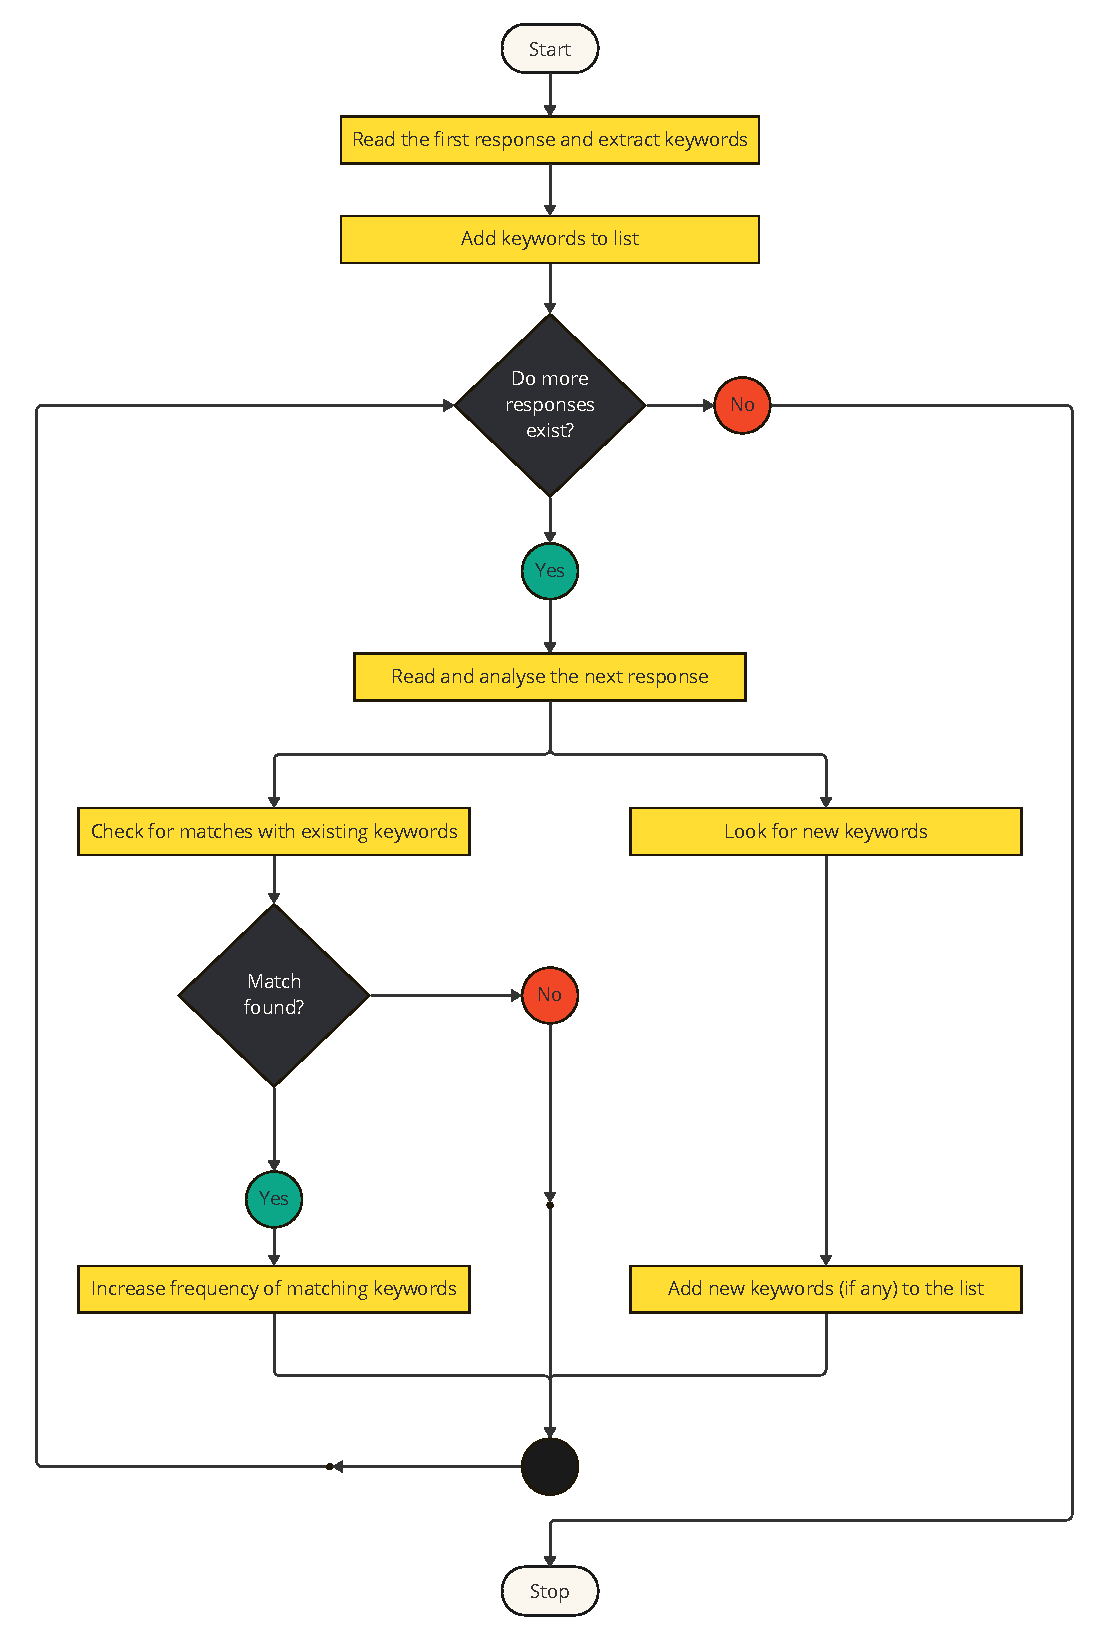
\includegraphics[width=0.6\textwidth]{figure/keyword_extraction_flowchart.pdf}
  \caption{Flowchart of the keyword extraction methodology employed.}
  \label{fig:kye_extraction}
\end{figure}


\subsection{Limitations and Ethical Considerations}

We ensured the ethical treatment of all participants throughout the research process, strictly adhering to GDPR guidelines to protect personal data and privacy. In line with these regulations, we made certain that no personal data was recorded at any stage of the survey. Participants were informed from the outset that their responses would remain completely anonymous, and we explicitly stated that no identifiable information would be collected. This was done to maintain the confidentiality of the data and to ensure participants felt secure in providing honest responses. Participation in the survey was entirely voluntary, with no questions marked as mandatory. This approach was designed to respect the autonomy of the respondents, allowing them to skip any questions they were uncomfortable answering without affecting their ability to submit the survey. 

Additionally, we offered participants the option to engage in a follow-up interview for more in-depth discussion. This option was also presented as entirely voluntary, and participants were given the choice to provide their contact details only if they were interested in participating further. This approach allowed us to gather richer qualitative data from those who were willing, while still respecting the privacy of those who chose not to engage further. One of the key limitations of our study was the decision not to record any identifying information about the participants, in order to comply with ethical standards and data protection regulations. While this ensured the anonymity and confidentiality of the respondents, it also introduced a significant limitation: we were unable to link responses back to specific individuals, countries, companies, or job positions. 

This lack of granularity in the data meant that while we knew which countries, companies, and positions were targeted, we could not directly associate specific responses with these variables. Consequently, our analysis could not account for potential differences in responses based on these factors, which may have provided additional insights into the impact of the pandemic on different segments of the supply chain. Another limitation was related to the survey design itself. Initially, we developed a more extensive set of questions, which we sent to a small group of known contacts for feedback. The feedback indicated that the survey was too lengthy, particularly given that participation was voluntary and there were no incentives offered. 

Respondents expressed reluctance to complete a long survey, which led us to significantly shorten the questionnaire. The final survey consisted of only 10 questions, with only 7 designed for quantitative analysis and 1 for qualitative analysis. This reduction in the number of questions limited the depth of the data we could collect, particularly in terms of more focused or detailed inquiries that might have provided richer insights. The trade-off, however, was an increased likelihood of participation, which was crucial given the challenges of obtaining responses without offering incentives.

Thus, while we took significant steps to ensure the ethical treatment of participants and to protect their privacy, these measures also introduced limitations in the scope and depth of our analysis. The constraints imposed by the need for anonymity, the voluntary nature of the survey, and the decision to limit the number of questions all impacted the breadth and specificity of the data collected. It should be noted that these limitations are acknowledged and should be considered when interpreting the findings of this study.

\section{The Interviews}

In our research, following the initial survey phase, we recognized the need for a more in-depth qualitative exploration to complement the limited data obtained (will be discussed in further sections) from the survey responses. The objective of this next methodological step was to conduct personal interviews with professionals who could offer deeper insights into the functioning of supply chains during the COVID-19 pandemic and the subsequent adjustments made in response to the challenges faced. Given the lower-than-expected response rate to our survey, despite our efforts to streamline the questions and ensure their relevance and ease of completion, we decided to pursue interviews as a means to bolster our research findings. 

Although our survey was carefully designed to minimize respondent burden—featuring voluntary participation, non-mandatory questions, and a concise structure—we observed that the engagement was insufficient to draw comprehensive conclusions from the quantitative data alone. To address this limitation and enhance the robustness of our research, we moved forward with conducting personal interviews. The initial plan to recruit interview participants involved leveraging the same pool of respondents from our survey. As previously mentioned, we included a question in the survey asking if participants were willing to engage in a follow-up interview for a more detailed discussion. Unfortunately, none of the survey respondents expressed interest in participating further, leaving us without candidates from the survey pool.

Consequently, we had to pivot our approach by once again reaching out to our professional networks, particularly through LinkedIn and other channels, to identify individuals who met the specific criteria required for the interview. It was essential that the interviewee had significant experience in the perishable goods sector and a background in supply chain management. This criterion was crucial to ensure that the insights provided during the interview were both relevant and valuable to our research. Consequently, this requirement also narrowed down people we could contact for the interview. After extensive outreach, we were able to secure a single interview with a participant whose qualifications were highly pertinent to our study. The individual in question had two years of direct experience in supply chain management at Nestlé, a leading company in the perishable goods industry. 

Additionally, the participant had professional experience with financial institutions such as S\&P. Academically, the interviewee held a master's degree in both finance and supply chain management, and a PhD in logistics supply chain, albeit with a focus on construction transport. At the time of the interview, the participant was employed as a Supply Chain Design Specialist at Volvo, adding a layer of credibility to the insights they provided.

% -------------------

Upon receiving agreement from the selected participant, one of the authors conducted the interview via an online Zoom meeting. Prior to the interview, the participant was fully informed of all ethical considerations, including the assurance that no personal data or personal information would be recorded or shared. The interview was conducted under the condition of anonymity, with the understanding that the participant's credentials would be disclosed to demonstrate their credibility and qualifications, but only with their explicit permission. The questions posed during the interview were carefully crafted based on the analysis of the survey data. Specifically, the questions were derived from the analysis of the multiple-choice questions using the PLS-SEM method, which will be elaborated upon in Section \ref{sec:pls-sem}, and from keyword analysis of the responses to subjective questions, as discussed in Section \ref{sec:keyword-analysis}. 

This ensured that the interview questions were directly relevant to the key points identified in the survey and allowed us to explore them in greater depth. In total, approximately 30 questions were prepared for the interview. However, it was understood that this list would serve as a flexible outline rather than a rigid script. The interview was designed to be conversational, allowing for the possibility of skipping certain questions or adding new ones depending on the flow of the discussion. Although no follow-up questions were pre-determined, the interview process included spontaneous follow-up questions to delve deeper into the insights provided by the participant. 

This flexibility was crucial in allowing the interviewer to explore the participant's responses more thoroughly and to gather more nuanced data. The questions covered a wide range of topics, from specific vulnerabilities within the supply chain to strategies for enhancing collaboration with suppliers and the role of technology in improving supply chain visibility and traceability. For example, one of the questions asked the participant to identify specific vulnerabilities within the supply chain, with a follow-up question probing whether they had encountered health-related problems in the food industry. Another question explored the flexibility and adaptability of the supply chain in responding to changes in demand or supply, with a follow-up asking for a specific example from the participant's experience.

The interview was conducted successfully, and the insights gathered provided valuable qualitative data that supplemented the quantitative findings from the survey. This data will be integrated into the overall analysis to provide a more comprehensive understanding of supply chain resilience during the pandemic. After the interview was completed, the actual list of questions and follow-up questions that were asked was compiled and can be found in Appendix \ref{appendix:interview}. This documentation ensures transparency in our methodology and allows for the replication of the study in future research. 

The interview conducted proved to be invaluable, offering detailed qualitative data that supplemented the limited quantitative results from our survey. The expertise and experience of the interviewee provided a depth of understanding that enriched our analysis, particularly regarding the resilience and adaptability of supply chains in the face of unprecedented disruptions like those caused by the COVID-19 pandemic. The insights gained from this interview will be discussed in further detail in the analysis and findings section of this paper, where we will integrate both the survey data and the qualitative insights to present a comprehensive view of the study's results.

% \todo[inline]{research process subsection to be added, where we summarise chronologically the entire process that was done}

\section{Survey Analysis: PLS-SEM}
\label{sec:pls-sem}

The aforementioned surveys and interviews yielded a total of \participantCount{} survey responses and one in-depth interviews. Current and following sections delineate the analytical methodologies employed to scrutinize the data obtained from these surveys and interviews.

In our study, we utilized SmartPLS 4 \parencite{smartpls2024} to analyze the structural equation model (SEM) based on the survey data collected. The constructs and hypotheses were operationalized through a series of survey questions, each carefully designed to measure specific aspects of the constructs in question. Below, we will elaborate on the process of model construction and the rationale behind the arrows and dependencies depicted in the Figure \ref{fig:constructs}. The survey data comprised questions targeted at measuring three main constructs: Pandemic Disruption, Change Management, and Resilience Effectiveness. Each of these constructs was associated with specific questions from the survey. For Pandemic Disruption, we used Question 4 which assesses the extent to which companies experienced supply chain disruptions due to the pandemic. 

This question serves as a critical indicator of the impact of COVID-19 on operational stability. Change Management was measured using Questions 5, 6, 8, 9, and 10. These questions capture various strategic responses implemented during the pandemic, including changes in supply management strategies, supplier diversification, creation of backup plans, adjustment of demand forecasting methods, and the presence of formal pandemic preparedness plans. These aspects collectively reflect the strategic adaptability and preparedness measures undertaken by companies in response to the pandemic. Resilience Effectiveness was gauged through Question 7, which evaluates the effectiveness of the company's resilience strategies such as inventory management and supplier diversification during the pandemic. This construct provides insights into how well existing strategies mitigated the pandemic's impact. The diagram also incorporates the specific survey questions associated with each construct, denoted by the yellow text boxes. For example, CMQ10, CMQ5, CMQ6, CMQ8, and CMQ9 represent the questions related to Change Management. The arrows pointing towards the Change Management node indicate the reflective measurement model, where each question (indicator) is influenced by the underlying construct. 

PLS-SEM analysis is well suited for various types of research data, some of them being the Likert Scale, which typically is a 5-point scale where respondents indicate their level of agreement or disagreement with a statement. The scales usually range from "Strongly Agree" to "Strongly Disagree", or similar. Likert scales are popular in measuring attitudes, perceptions, and behavioral intentions. It is also suited for Binary or Dichotomous Scales, which are simple yes/no or true/false responses. In our case, the responses for Questions 4 and 7 are in the Likert Scale and the responses for Questions 5, 6, 8, 9 and 10 are within the Binary Scale. This is briefly described below.

\subsection{The analysis process}

\begin{enumerate}

    \item \textbf{Selection of Questions for Analysis:} To apply PLS-SEM, we selected questions 4 to 10 for analysis. These questions were chosen because they are either yes/no questions or questions with answers on a scale ranging from 0 to 5, which are suitable for the PLS-SEM modeling approach.

    \item \textbf{Construct Development:} Constructs are developed based on the questions asked, specifically questions 4-10, to create meaningful hypotheses. Constructs represent the theoretical concepts that underpin the variables of interest in the study.

    \item \textbf{Hypothesis Creation and Validation:} The primary objective is to formulate hypotheses based on the research questions and subsequently validate or invalidate them using the responses received. The validation will be conducted through the results obtained from the PLS-SEM analysis.

\end{enumerate}


\subsection*{Summary:}
\noindent Here we will summarise the aforementioned process.

\begin{itemize}
    \item \textbf{Step 1:} Select objective questions (Questions 4-10).
    \item \textbf{Step 2:} Develop constructs based on the selected questions.
    \item \textbf{Step 3:} Formulate hypotheses related to the developed constructs.
    \item \textbf{Step 4:} Apply PLS-SEM to analyze the data and obtain results.
    \item \textbf{Step 5:} Validate or invalidate the hypotheses based on the analysis results.
\end{itemize}

\subsection{Constructs Developed}

Based on the selected questions, we have developed a total of three constructs by grouping similar questions. Each construct is designed to measure different dimensions of supply chain resilience in the context of the COVID-19 pandemic. The constructs and their corresponding rationale are as follows:

\begin{itemize}

    \item \textbf{Construct 1: Pandemic Disruption}
    \begin{itemize}
        \item \textbf{Question Used:} Question 4
        \item This construct is derived from a question that assesses the extent of disruption experienced by companies in their supply chain due to the pandemic. It serves as an indicator of the overall impact of COVID-19 on business operations and highlights the vulnerabilities within supply chains during this period.
    \end{itemize}

    \item \textbf{Construct 2: Change Management}
    \begin{itemize}
        \item \textbf{Questions Used:} Questions 5, 6, 8, 9, 10
        \item This construct is based on multiple questions that address various changes implemented in response to the pandemic. These include adjustments in management strategies, diversification of suppliers, creation of backup plans, modification of forecasting methods, and the establishment of formal preparedness plans. Together, these questions capture the strategic adaptability and proactive measures adopted by companies to manage pandemic-induced disruptions.
    \end{itemize}

    \item \textbf{Construct 3: Resilience Effectiveness}
    \begin{itemize}
        \item \textbf{Question Used:} Question 7
        \item This construct focuses on evaluating the effectiveness of the resilience strategies employed by companies during the pandemic, such as inventory management and supplier diversification. It provides insights into how well these strategies mitigated the impact of disruptions and contributed to overall supply chain resilience.
    \end{itemize}

\end{itemize}


\begin{figure}[H]
  \centering
  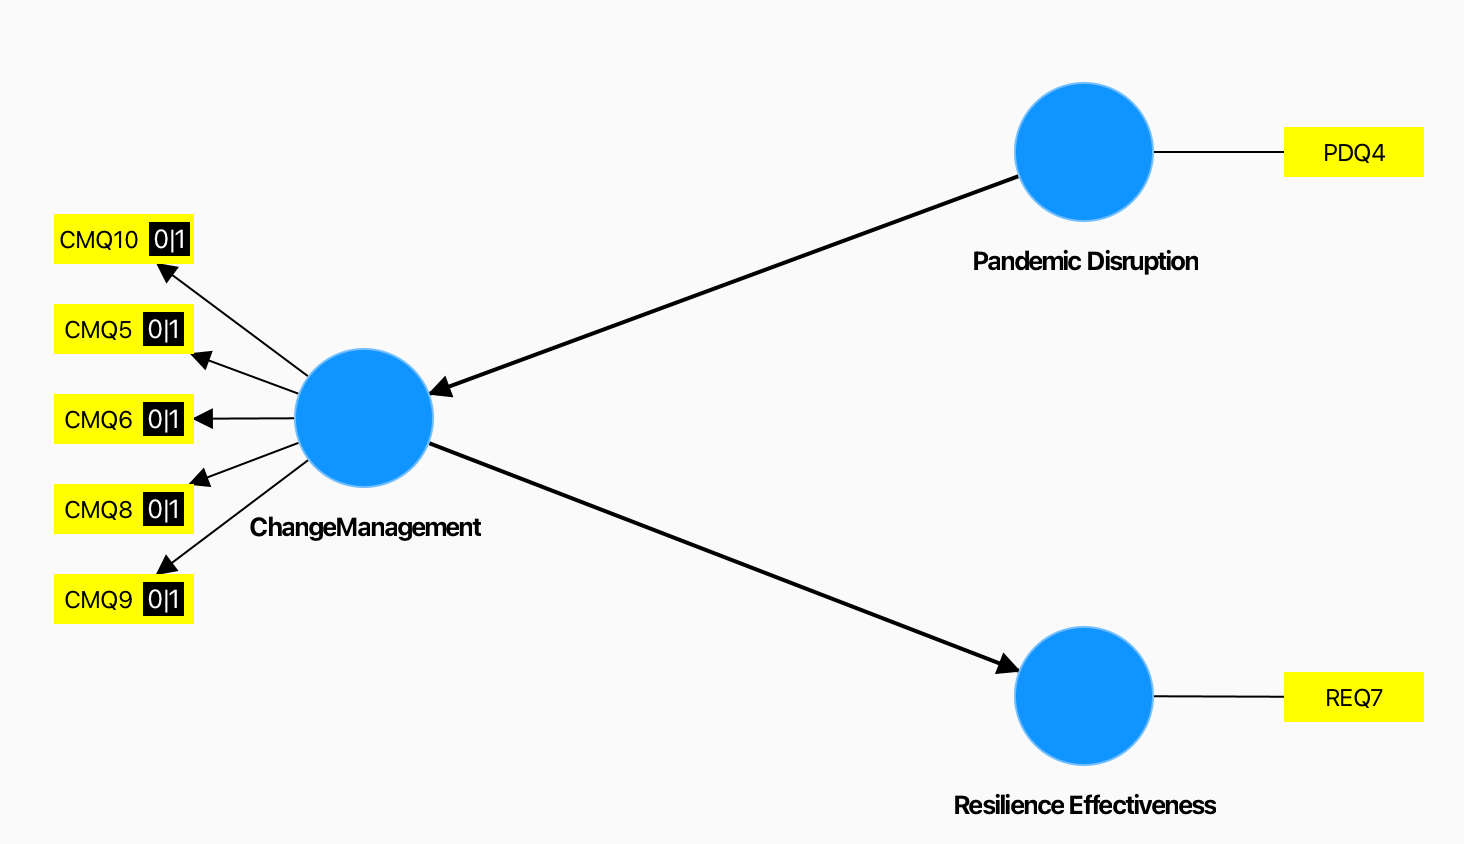
\includegraphics[width=1\textwidth]{figure/initial_model.png}
  \caption{Structural Model in SmartPLS showing the relationships between constructs. The model includes Pandemic Disruption (Q4), Change Management (Q5, Q6, Q8, Q9, 10), and Resilience Effectiveness (Q7). Arrows indicate hypothesized dependencies: Pandemic Disruption's impact on Change Management and Resilience Effectiveness, and Resilience Effectiveness's influence on Change Management. $[0|1]$ Adjacent to the question numbers indicate the binary nature of the questions. Other questions belong to the Likert Scale.}
  \label{fig:constructs}
\end{figure}


\noindent Using SmartPLS 4, we constructed a model (Figure \ref{fig:constructs}) to test our hypotheses. The structural model posits the following relationships:

\begin{enumerate}
    \item \textbf{Pandemic Disruption leads to Change Management (H1)}: This hypothesis suggests that higher levels of disruption due to the pandemic are positively associated with an increase in change management strategies. The arrow from Pandemic Disruption to Change Management in the diagram represents this hypothesis. The rationale is that significant disruptions necessitate strategic changes to adapt and mitigate the impact.

    \item \textbf{Resilience Effectiveness reduces the need for extensive Change Management (H2)}: This hypothesis proposes a negative relationship between the effectiveness of resilience strategies and the extent of change management. If a company’s existing resilience strategies are effective, it may not need to implement extensive changes. This is depicted by the arrow from Resilience Effectiveness to Change Management, indicating that effective resilience strategies can mitigate the need for further change.

    \item \textbf{Pandemic Disruption influences Resilience Effectiveness (H3)}: This hypothesis posits a positive relationship between the level of pandemic disruption and the perceived effectiveness of resilience strategies. Higher levels of disruption may prompt companies to evaluate and enhance their resilience strategies, thus leading to higher effectiveness. This relationship is shown by the arrow from Pandemic Disruption to Resilience Effectiveness in the diagram.

\end{enumerate}

Upon conducting the analysis using the SmartPLS tool for PLS-SEM, we can evaluate the validity of our hypothesized relationships among the constructs. By examining the path coefficients, significance levels (p-values), and the R² values for each endogenous construct, SmartPLS provides comprehensive insights into the strength and significance of the proposed causal paths. In our specific case, this involves assessing whether the hypothesized positive relationship between Pandemic Disruption and Change Management, the negative relationship between Resilience Effectiveness and Change Management, and the positive relationship between Pandemic Disruption and Resilience Effectiveness hold true. 

Additionally, the bootstrapping procedure available in SmartPLS allows us to obtain estimates of standard errors and confidence intervals, further solidifying our hypothesis testing. The evaluation of the model fit indices, such as the SRMR (Standardized Root Mean Square Residual), will help determine the overall adequacy of our model, enabling us to conclude whether the empirical data supports our theoretical propositions. Thus, the detailed results obtained from SmartPLS will enable us to confirm or refute our hypotheses with a considerable degree of statistical confidence. In configuring the SmartPLS software for our PLS-SEM analysis, several key settings were chosen to ensure interpretable results. We selected the Principal Component Analysis (PCA) weighting scheme, a common default choice, as it uses the first principal component of the block’s indicators as the composite score, providing a reliable and standard approach. To facilitate easier interpretation of path coefficients and enable comparisons across constructs, we opted for standardized results, which convert all variables to a common scale. 

For the initial weights, we adhered to the algorithm’s default settings. Regarding the handling of missing values, considering that only one response was partially missing, we utilized casewise deletion, provided it did not significantly reduce our sample size below acceptable limits for robust analysis. Lastly, we did not apply any additional weighting vectors, as none were necessary for our analysis.

\section{Survey Analysis: Keyword Extraction}
\label{sec:keyword-analysis}

The analysis resulted in 10 keywords which were used the most by all our survey-takers. The first round of elimination was to use a cut off of all the words which have less than 5 occurrences. Through this cut off we could make sure that the words that have been chosen for keyword analysis were really the words that had significance for our survey subjects. This resulted in 21 keywords that were chosen for the next round of analysis/elimination. The next round was more based on the context and similarity of the wording used by our survey subjects. For example, words such as "perishable" and "meat and dairy", and/or vegetables are categorized as a single keyword and the frequencies were added to get a cumulative number. Other words such as "demand forecasting" and "strategic foresight" were also put together to add their number of occurrence and shorten our list of keywords. Finally after this process of contextual analysis we ended up with 10 most important keywords which were used by our survey subjects which are stated in Table \ref{tab:keyword-frequency} in order of their significance of occurrence.

\begin{table}[h!]
\centering
\begin{tabular}{|c|c|}
\toprule
\textbf{Keyword} & \textbf{Frequency} \\ 
\midrule
Resilience & 41 \\ 
\hline
Diversified Supplier Base & 30 \\
\hline
Innovation & 27 \\
\hline
Operational Continuity & 26 \\
\hline
Demand Forecasting & 25 \\ 
\hline
Adaptability & 25 \\ 
\hline
Sustainability & 18 \\ 
\hline
Pandemic-induced Supply Chain Disruptions & 13 \\ 
\hline
Agility & 12 \\ 
\hline
Perishables & 12 \\ 
\bottomrule
\end{tabular}
\caption{Frequency of Keywords Related to Supply Chain Resilience}
\label{tab:keyword-frequency}
\end{table}

Using these keywords we came up with 20 i.e. 2 interview questions per keyword to be able to interview our interviewees and understand their input on these significant keywords in our survey and understand their thoughts on these subjects. For this we studied several research papers to come up with interview questions relevant to the topics focused on our keywords \parencite{Tukamuhabwa2015SupplyStudy,Ponomarov2009UnderstandingResilience,Wu2007MethodologyAnalysis,Sawik2017AManagement,Chowdhury2021COVID-19Review}. To be able to prepare for the interview we followed the guidance provided by \textcite{Ghauri2020ResearchStudies} to perform the pre-interview, interview, and post-interview preparation and develop our skills on interviewing our subjects.

\section{Analysis of Long Form Interviews}
\label{sec:intervew-analysis}

The purpose of this interview analysis is to delve deeply into the experiences and insights shared by a supply chain professional to explore the various dimensions of supply chain resilience in the context of the COVID-19 pandemic. By systematically evaluating the interviewee's responses, we seek to validate or invalidate our hypotheses concerning the immediate impacts of the pandemic on supply chains and the strategies implemented by companies to mitigate these impacts and prepare for future crises. The insights gathered from this interview are crucial in validating our hypotheses, specifically those related to the challenges faced by suppliers of perishable goods during the pandemic and the strategies adopted to enhance supply chain resilience. Through the interview, we explore the interviewee's perspective on whether suppliers faced significant disruptions \textit{(Hypothesis 1)}. Additionally, we aim to understand whether these suppliers implemented new strategies to enhance resilience \textit{(Hypothesis 2)}. 
The relevance of this interview is emphasized by the interviewee's substantial experience in managing supply chains for perishable goods. With direct experience in supply chain management at Nestlé, a leading company in the perishable goods industry, and a current role as a Supply Chain Design Specialist at Volvo, the interviewee brings a nuanced perspective that bridges both practical and theoretical knowledge. Their academic qualifications, including a PhD in logistics supply chain and master’s degrees in finance and supply chain management, further enhance the credibility of their insights, particularly concerning complex supply chain dynamics and the need for adaptive strategies during crises. Moreover, the interviewee's background in both the perishable goods sector and broader supply chain management offers a unique vantage point to explore how companies have responded to the disruptions caused by the COVID-19 pandemic.

\subsection{Initial Challenges Faced by Suppliers of Perishable Goods}

The interview reveals several critical challenges that suppliers of perishable goods encountered during the COVID-19 pandemic, which align with the hypotheses proposed in our research. The interviewee described the pandemic period as a time of substantial difficulty, stating, “\textit{it was a great challenge for supply chain management because we have a global supply chain. So it was like really difficult to source the raw material and then send the finished product to the customers}.” This observation supports \textit{Hypothesis 1}, which asserts that suppliers of perishable goods faced significant disruptions in their supply chains due to the pandemic.

\subsubsection{Supply Shortages and Delays in Transportation}

The interviewee highlighted several immediate impacts on supply chains, including supply shortages and delays in transportation. One of the prominent examples mentioned was the incident at the Suez Canal, where “\textit{pirates...stopped the Canal, and it created a big challenge on how to fix it and how to send products through there}.” It is important to note that we could not find any significant incident involving pirates blocking the Suez Canal. However, we assume the interviewee may have mixed it up with the Ever Given incident in 2021, where a massive container ship ran aground, blocking the Suez Canal for nearly a week. This blockage led to a substantial global trade disruption, with an estimated daily loss of \$9.6 billion \parencite{Harper2021SuezDay}, critically affecting regions such as Dubai, where “\textit{all the material goes from that path...that area got critically affected because it got closed down for a long period of time}.” The incident illustrates the vulnerability of supply chains that rely heavily on specific transit routes, supporting the notion that external disruptions, such as geographical bottlenecks, can have a profound impact on the ability of suppliers to meet demand. Furthermore, the interviewee pointed out the complexities associated with managing delays caused by transportation issues. They stated, “\textit{it is really a challenge, like how we can meet the demand and...how much time before you have to place the order to incorporate in-transit time, transport time}.” This statement indicates that unpredictable delays created significant bottlenecks in the supply chain, requiring companies to re-calibrate their logistics and inventory management strategies frequently. These challenges, stemming from transportation delays and route blockages, provide strong evidence for Hypothesis 1, which posits that suppliers experienced considerable disruptions.

\subsubsection{Labor Constraints and Increased Costs}

In addition to supply shortages and transportation delays, labor constraints emerged as a significant challenge during the pandemic. Although the interviewee did not directly elaborate on labor issues, it is implied through their references to challenges in maintaining operations and managing increased costs. The global nature of supply chains meant that suppliers faced difficulties in both “\textit{sourcing the raw material and sending the finished product to the customers},” suggesting disruptions not only in material availability but also in the workforce needed to process and transport these materials. The increased need for labor to manage these disruptions, coupled with constraints due to health and safety regulations, likely resulted in additional costs, further complicating the supply chain management process.

\subsubsection{Comparative Analysis with Hypotheses}

Comparing these accounts with \textit{Hypotheses 1} provides a clear indication that Hypothesis 1 is more strongly supported by the interview data. The interviewee's experiences emphasizes significant disruptions in supply chains due to several factors, including logistical challenges, transportation delays, and supply shortages. Additionally, the arguments posed suggests that suppliers of perishable goods did not experience substantial disruptions. The cumulative impact of incidents like the Suez Canal blockage, coupled with the complexities of global supply chain management during a pandemic, illustrates that the disruptions were indeed significant and widespread.

\subsubsection{Specific Examples Illustrating Disruptions}

Several specific examples from the interview point out the types of disruptions encountered by suppliers. The Suez Canal incident, in particular, serves as a prime example of a transportation-related disruption that significantly affected supply chains. The interviewee mentioned that the closure of the canal had a "critical impact on the Dubai market," and the subsequent difficulty in “\textit{meeting demand}” illustrates the dependency of regional markets on specific supply routes. Moreover, the example highlights how disruptions in one part of the supply chain can have cascading effects across various regions, demonstrating the interconnectedness and fragility of global supply chains. Additionally, the interviewee referred to the broader challenges of managing supply chain operations amid the pandemic, emphasizing the need for “\textit{correct demand forecasting}” to prevent bottlenecks. This statement reflects the inherent difficulty in managing supply chains under uncertain conditions, where disruptions can occur suddenly and unpredictably. The reliance on accurate demand forecasting becomes even more critical in such scenarios to avoid excess inventory or stockouts, further supporting the notion of significant disruptions in supply chains during the pandemic. 

This account provides substantial evidence that suppliers of perishable goods faced multiple initial challenges during the COVID-19 pandemic, including supply shortages, transportation delays, labor constraints, and increased costs. These challenges align closely with \textit{Hypothesis 1}, suggesting that significant disruptions were experienced by suppliers. The examples provided, such as the Suez Canal blockage and regional market dependencies, illustrate the fragility of global supply chains and the cascading impact of localized disruptions. Therefore, the initial analysis strongly supports the argument that the pandemic had a profound and widespread impact on supply chain operations for suppliers of perishable goods.

%===================3rd Section

\subsection{Strategies Adopted by Suppliers During the Pandemic}

The interview provides an overview of both immediate and long-term strategies adopted by suppliers of perishable goods in response to the disruptions caused by the COVID-19 pandemic. These strategies were crucial for maintaining supply chain resilience and ensuring the continuous flow of goods, despite unprecedented challenges.

\subsubsection{Immediate Response Strategies}

The interviewee detailed several short-term strategies employed by suppliers to cope with the immediate disruptions caused by the pandemic. One key strategy was sourcing alternatives, as the interviewee noted, “\textit{it was really difficult to source the raw material and then send the finished product to the customers}.” This difficulty led companies to diversify their supply base to reduce dependency on single sources. The interviewee emphasized the importance of local partnerships, suggesting that “\textit{we should have more supply partnerships in local markets… so our reliance will not become our sole responsibility}.” This reflects a strategic pivot towards sourcing materials from more geographically proximate suppliers, thereby reducing the risk associated with long-distance supply chains.

Additionally, there was a significant focus on using local warehouses to mitigate disruptions in global supply chains. The interviewee mentioned that companies began to “\textit{consider the concept of local warehouses… because they are closer to where things are needed}.” This strategy aligns with \textit{Hypothesis 2}, which posits that suppliers of perishable goods have implemented new strategies and procedures to enhance supply chain resilience. By utilising local warehouses, suppliers could reduce transportation time and costs while increasing the speed of response to sudden changes in demand. The diversification of suppliers also played a critical role in managing risks. 

The interviewee highlighted the benefits of having a combination of large and small suppliers, noting that “\textit{small suppliers are more flexible, whereas larger suppliers are often less adaptable}.” This mix allowed companies to benefit from the flexibility and adaptability of smaller suppliers while still maintaining relationships with larger, more established suppliers for bulk procurement needs. This diversification strategy is consistent with the need for flexibility in responding to disruptions, as outlined in \textit{Hypothesis 2}. Additionally, suppliers enhanced collaboration with both small and large suppliers to manage risks better. As the interviewee noted, “\textit{there should be collaborative partnerships and more involvement of different stakeholders}.” 

This approach enabled suppliers to share risks and responsibilities, fostering a more resilient supply chain network. For example, the interviewee described the increased use of third-party transporters and more flexible transport terms, which allowed suppliers to adapt quickly to changing circumstances. The inclusion of third-party logistics providers facilitated a more agile and responsive supply chain, capable of overcoming sudden transportation challenges or bottlenecks.

\subsubsection{Long-Term Strategic Changes}

In addition to immediate responses, companies made several longer-term strategic changes to enhance supply chain resilience. The interviewee noted that technology adoption became a key focus, with companies looking to integrate technologies such as the Internet of Things (IoT) and Artificial Intelligence (AI) into their supply chains. These technologies were seen as crucial for “\textit{tracking and traceability of the products in real-time},” which is vital for managing perishable goods that require strict monitoring of storage conditions and transportation timelines. The use of IoT and AI could help “\textit{resolve all the bottlenecks and buffer stocks and safety stocks}” by providing real-time data and insights, enabling companies to make more informed decisions quickly. However, it is important to note that the interviewee acknowledged a lack of expertise in computer science or related technical fields, resulting in a limited understanding of AI and IoT. 

Moving on, the interviewee also highlighted the development of new supplier partnerships and a shift towards more comprehensive contingency planning. After the pandemic, many companies began to establish crisis management teams whose “\textit{sole job is to understand and work only on alternative solutions}.” This move illustrates a proactive approach to preparedness, ensuring that companies are better equipped to handle future disruptions. Such investments in crisis management and planning are consistent with \textit{Hypothesis 2}, which suggests that suppliers have implemented new strategies to enhance their resilience.

Additionally, the interview data suggests that several suppliers have indeed made substantial changes, such as adopting new technologies and establishing dedicated crisis management teams. The shift towards technology adoption and the development of new supplier partnerships indicate that companies are actively seeking to enhance their supply chain resilience in preparation for future pandemics or similar disruptive events. The interviewee also discussed the importance of continuous assessment and finding new suppliers to improve terms and conditions and maintain supply chain agility. They stated, “\textit{it is always good to keep looking for new suppliers, innovative ways, and new ways of transporting products}.” This approach reflects a commitment to dynamic supply chain management, where constant evaluation and adjustment are necessary to mitigate risks and respond to changing circumstances.

\subsubsection{Strategies Adopted - Summary}

Thus, the interview reveals that suppliers of perishable goods adopted a range of both immediate and long-term strategies to enhance supply chain resilience during the COVID-19 pandemic. Short-term strategies included sourcing alternatives, local warehousing, supplier diversification, and enhanced collaboration with third-party transporters. Long-term strategic changes focused on technology adoption, new supplier partnerships, and contingency planning. These actions align strongly with \textit{Hypothesis 2}, demonstrating a proactive approach to resilience and preparedness.

%=================SECTION 4

\subsection{Exploring Additional Themes}

\subsubsection{Flexibility and Adaptability of Supply Chains}
The interviewee highlighted the importance of flexibility and adaptability in supply chains, especially in response to uncertain demand changes during the pandemic. One of the key strategies mentioned was the adoption of a Just-In-Time (JIT) approach to inventory management, particularly for perishable goods. The interviewee explained, \textit{“we cannot even build more stock. So then the idea was to reduce the time when the item is in inventory, using more of a Just-In-Time kind of approach."} This method allowed companies to minimize inventory holding times, thereby reducing the risk of spoilage and wastage, which is critical for perishable goods. The flexibility of supply chains was further enhanced by employing more adaptable transportation methods and diversifying transport partners. For instance, the interviewee mentioned that during the pandemic, they “added actually more third-party transporters so that [they] meet [their] customer requirement.” 

This strategy ensured that the supply chain remained responsive to fluctuating demands and unforeseen disruptions.  These measures are essential for enhancing the overall resilience of supply chains. By adopting adaptable inventory management and transportation strategies, companies can better withstand disruptions and respond more effectively to sudden changes in demand or supply. These insights are directly aligned with the research question, which seeks to understand how suppliers of perishable goods enhance their resilience during and after pandemics.

\subsubsection{Role of Technology and Digitalization}
The interviewee also emphasized the role of digital platforms in enhancing supply chain resilience. The use of digital platforms was suggested as a means to improve real-time communication and coordination among stakeholders. The interviewee noted, “if there will be a shared digital platform… it is easy to access, everybody can access it and also it will be real-time." This could significantly improve the responsiveness and transparency of supply chains, allowing for quicker adjustments to changing circumstances. Furthermore, the interviewee identified the potential of digital platforms in fostering collaboration and joint risk management, particularly in crisis situations like the pandemic. Despite recognizing the benefits, the interviewee also acknowledged challenges, such as the need for standardization across markets and the complexity of integrating such platforms into existing systems. These observations emphasize both the potential advantages and the implementation challenges of digital solutions in supply chain management for perishable goods.

\subsubsection{Collaboration and Communication Challenges}
Collaboration and communication among suppliers, partners, and other stakeholders were highlighted as crucial for enhancing supply chain resilience. The interviewee pointed out several examples of poor communication and lack of coordination that created inefficiencies. For example, they mentioned, “the transporter doesn’t communicate with the materials, the receiver… [leading to] inefficiencies,” and similarly, “the factory doesn’t communicate… what is their production schedule or what is their capacity." Such breakdowns in communication led to mismatches in supply and demand and contributed to delays and waste. To mitigate these issues, the interviewee suggested the adoption of shared digital platforms to facilitate real-time communication and transparency. This aligns with their earlier point about technology adoption, emphasizing the need for integrated systems that provide all stakeholders with access to relevant information in real time. The interviewee recommended, “regular communication channels… shared responsibility or shared performance measures or some decision-making process,” which would foster joint planning and ensure that all parties are aligned in their goals and responses to disruptions.

\subsubsection{Insights}

The interview provided valuable insights into the challenges faced by suppliers of perishable goods during the COVID-19 pandemic and the strategies implemented to enhance supply chain resilience. The interviewee's experiences confirmed that significant disruptions occurred, validating Hypothesis 1. The evidence also demonstrated that companies adopted various strategies, both short-term and long-term, to address these disruptions, supporting Hypothesis 2. Additional insights emerged regarding the critical role of flexibility and adaptability in supply chains, particularly in response to unpredictable demand changes and the importance of Just-In-Time inventory strategies. The interview also highlighted the need for enhanced communication and collaboration among supply chain stakeholders to improve transparency and trust, suggesting the use of shared digital platforms for real-time information sharing.

Additionally, the interview also pointed to several areas where further research is needed. For example, future studies could explore the practical challenges and feasibility of implementing advanced technologies, such as IoT and AI, in the supply chains of perishable goods. Moreover, further research could examine the long-term impacts of these strategic changes on supply chain resilience and performance in different geographic and market contexts.

